% Compile the document by command 'latex model.tex' in the terminal. You can turn the dvi file into a postscript file by using the command dvips, and generate a pdf file either by dvipdf or ps2pdf. 
\documentclass[a4paper,10pt]{article}
% Use latin1 in Unix and [ansinew] in Windows
%\usepackage[latin1]{inputenc}
\usepackage[utf8]{inputenc}
% This includes letters such as  and 
\usepackage[T1]{fontenc}
% Use here 'Finnish' for Finnish hyphenation. You may have to compile the code twice after the change. 
\usepackage[english]{babel}
%\usepackage[finnish]{babel}
% For postscript figures
\usepackage[pdftex]{graphicx}
% Some math stuff
\usepackage{amsmath,amsfonts,amssymb,amsbsy}  
% This is just to include the urls
\usepackage{hyperref}
\usepackage[nottoc]{tocbibind}
\usepackage[titletoc]{appendix}
\usepackage{moreverb}

\begin{document}

\title{AS-84.3144 Field and Service Robotics\\Project Report}
\author{Group 3:\\Pekka Heikkilä, Konsta Hölttä, Antti Kangasrääsiö,\\Toni Liski, Iiris Routa, Hanna Ukkola, Quentin Verleysen}

\maketitle
\thispagestyle{empty}
\newpage
\tableofcontents
\newpage
%\pagestyle{plain}
%\pagenumbering{arabic}
\section{Introduction}

In this project we developed software and a manipulator for an autonomous sample collection mobile robot. We used J2B2, a ready made differential wheeled robot with a caster wheel as the platform for which to create our applications. The task of the robot was to search and map an unknown flat indoor area to find interesting objects and bring them to a specified goal area. The robot needed to be able to spot and avoid walls and other obstacles and distinguish unwanted objects from targets during its mission.

The target objects were red half-spheres and the unwanted objects otherwise similar but green half-spheres. The goal area was the same area where the robot started its mission. The mission time was 15 minutes. The robot used bumpers, a laser range finder and a camera for environment perception.

In this report we introduce our solution for the robot's program architecture and describe each subsystem in detail. We present our results and analyse the process of developing our solution. As a conclusion we give some critique for the process and analyse our outcomes.

\section{Program architecture}

The program is divided in several small parts that work together. The major parts are visualized in picture \ref{softwarearch}. Everything starts from a main program similar to the given demo. It initializes the J2B2 interfaces and a main class called Robot.

Robot then starts several threads for things that need to run simultaneously and must not block each other from fast actions. The main program enters a loop that runs until the user quits it.

The biggest separate parts of the program are: planner, SLAM, navigation, motion control, and the main program that connects all these. The main program, Robot, contains the logic for the planner, and controls the other modules.

\subsection{Threading}

The program spawns six threads: main planning, sensing, motor state updating, slam, camera, and debug graphics ("user interface"). Especially the slam and camera algorithms take time, and it’s critical that the control loops run fast.

The sensing thread asks the J2B2 interface for new information and stores it in variables that are in the scope of the main program. Some of the data cannot be read or written atomically, which is why the measurements are protected by locks (inherited from CSync). Each measurement type has its own lock that must be held when reading or writing the data.

\subsection{Data flow}

\begin{figure}[h]	% Use here 'h' for 'here', 't' for 'top' or 'b' for bottom. '!' makes the figure float.
\begin{center}
\includegraphics[width=10.0cm]{architecture.png}
\caption{Rough program architecture and data flow directions.}
\label{softwarearch} % The label for the figure. You can refer to the figure by \ref{fig:1} in the text. 
\end{center}
\end{figure}

Refer to \ref{softwarearch} for visualizations.

SLAM takes the laser and odometry data first, and other parts of the program get the location from SLAM. The camera data is read by the camera thread straight from the robot interfaces, not via SLAM. It tries to find spheres and the target area from the pictures. When something is found, it tells SLAM about that.

The planner decides what to do at each point of time and transfers information between some of the modules. For example, navigation doesn’t talk directly to SLAM, but the planner asks the current location from SLAM and gives it as a starting point to navigation when a route from current point to somewhere is needed. The route midpoints are transferred from the navigation module to the motion control module.

Some of the data moves through the main program instead of directly from one module to other (some small parts of some modules in the figure are actually scattered around several classes or files). This way the modules' classes do not need to store references to each other; they just are contained in the main program, which then decides what to do.

\section{Coding}

The code was written thoroughly in C++ and developed with the help of the version control system called Git \cite{git}. A central repository was used, but users wrote also local tests without the need of publishing everything, thanks to Git's distributed model. Several branches were used at the same time to help parallel development of separate features, and total number of commits in the master branch is about 200.

A detailed set of programming guidelines were decided. In the beginning, code quality was very good and modular. Much of the code was written during the last moments in a hurry, though, and not all of the rules were adhered to. The main modules could have separated their logic into smaller classes to ease the development, but that was not necessary as the development did not really last long.

\section{SLAM}

\subsection{Introduction}

The purpose of the SLAM module is to form a map of the surrounding area of the robot and to keep track of the location of the robot in it. The SLAM module is also responsible for offering functions that can visualize the relevant data if needed.

The module performs this task by receiving three types of information from other modules: odometry data, laser range data and formatted image data. The other modules can request a reference to the most current MapData object, which is an encapsulation of all the relevant data concerning the environment and the robot's location in it. The other modules can also ask the module to visualize the current data using a given SDL screen object.

For the main SLAM functionality, the module uses a Rao-Blackwellian particle filter, which is implemented by the external gmapping library \cite{gmapping_home}. All other functionality is programmed by the group (mainly Antti).

This section will explain the architecture of the SLAM module as well as a short introduction to the used external gmapping algorithm. Some of the main algorithms that were used for performing the above tasks are presented in more detail in appendix \ref{apA}.

\subsection{Module Architecture}

The module consists of three main classes: SLAM, MapData and GFSJ2B2. In addition to these, there are four additional helper classes and enumerations used for data abstraction: RobotLocation, Location, GridPoint, ImageData and ObservationType. The classes are illustrated in figure \ref{slam_classes}.

This subsection will discuss the classes in more detail, as well as a description of how the module works as a whole.

\begin{figure}[h]	% Use here 'h' for 'here', 't' for 'top' or 'b' for bottom. '!' makes the figure float.
\begin{center}
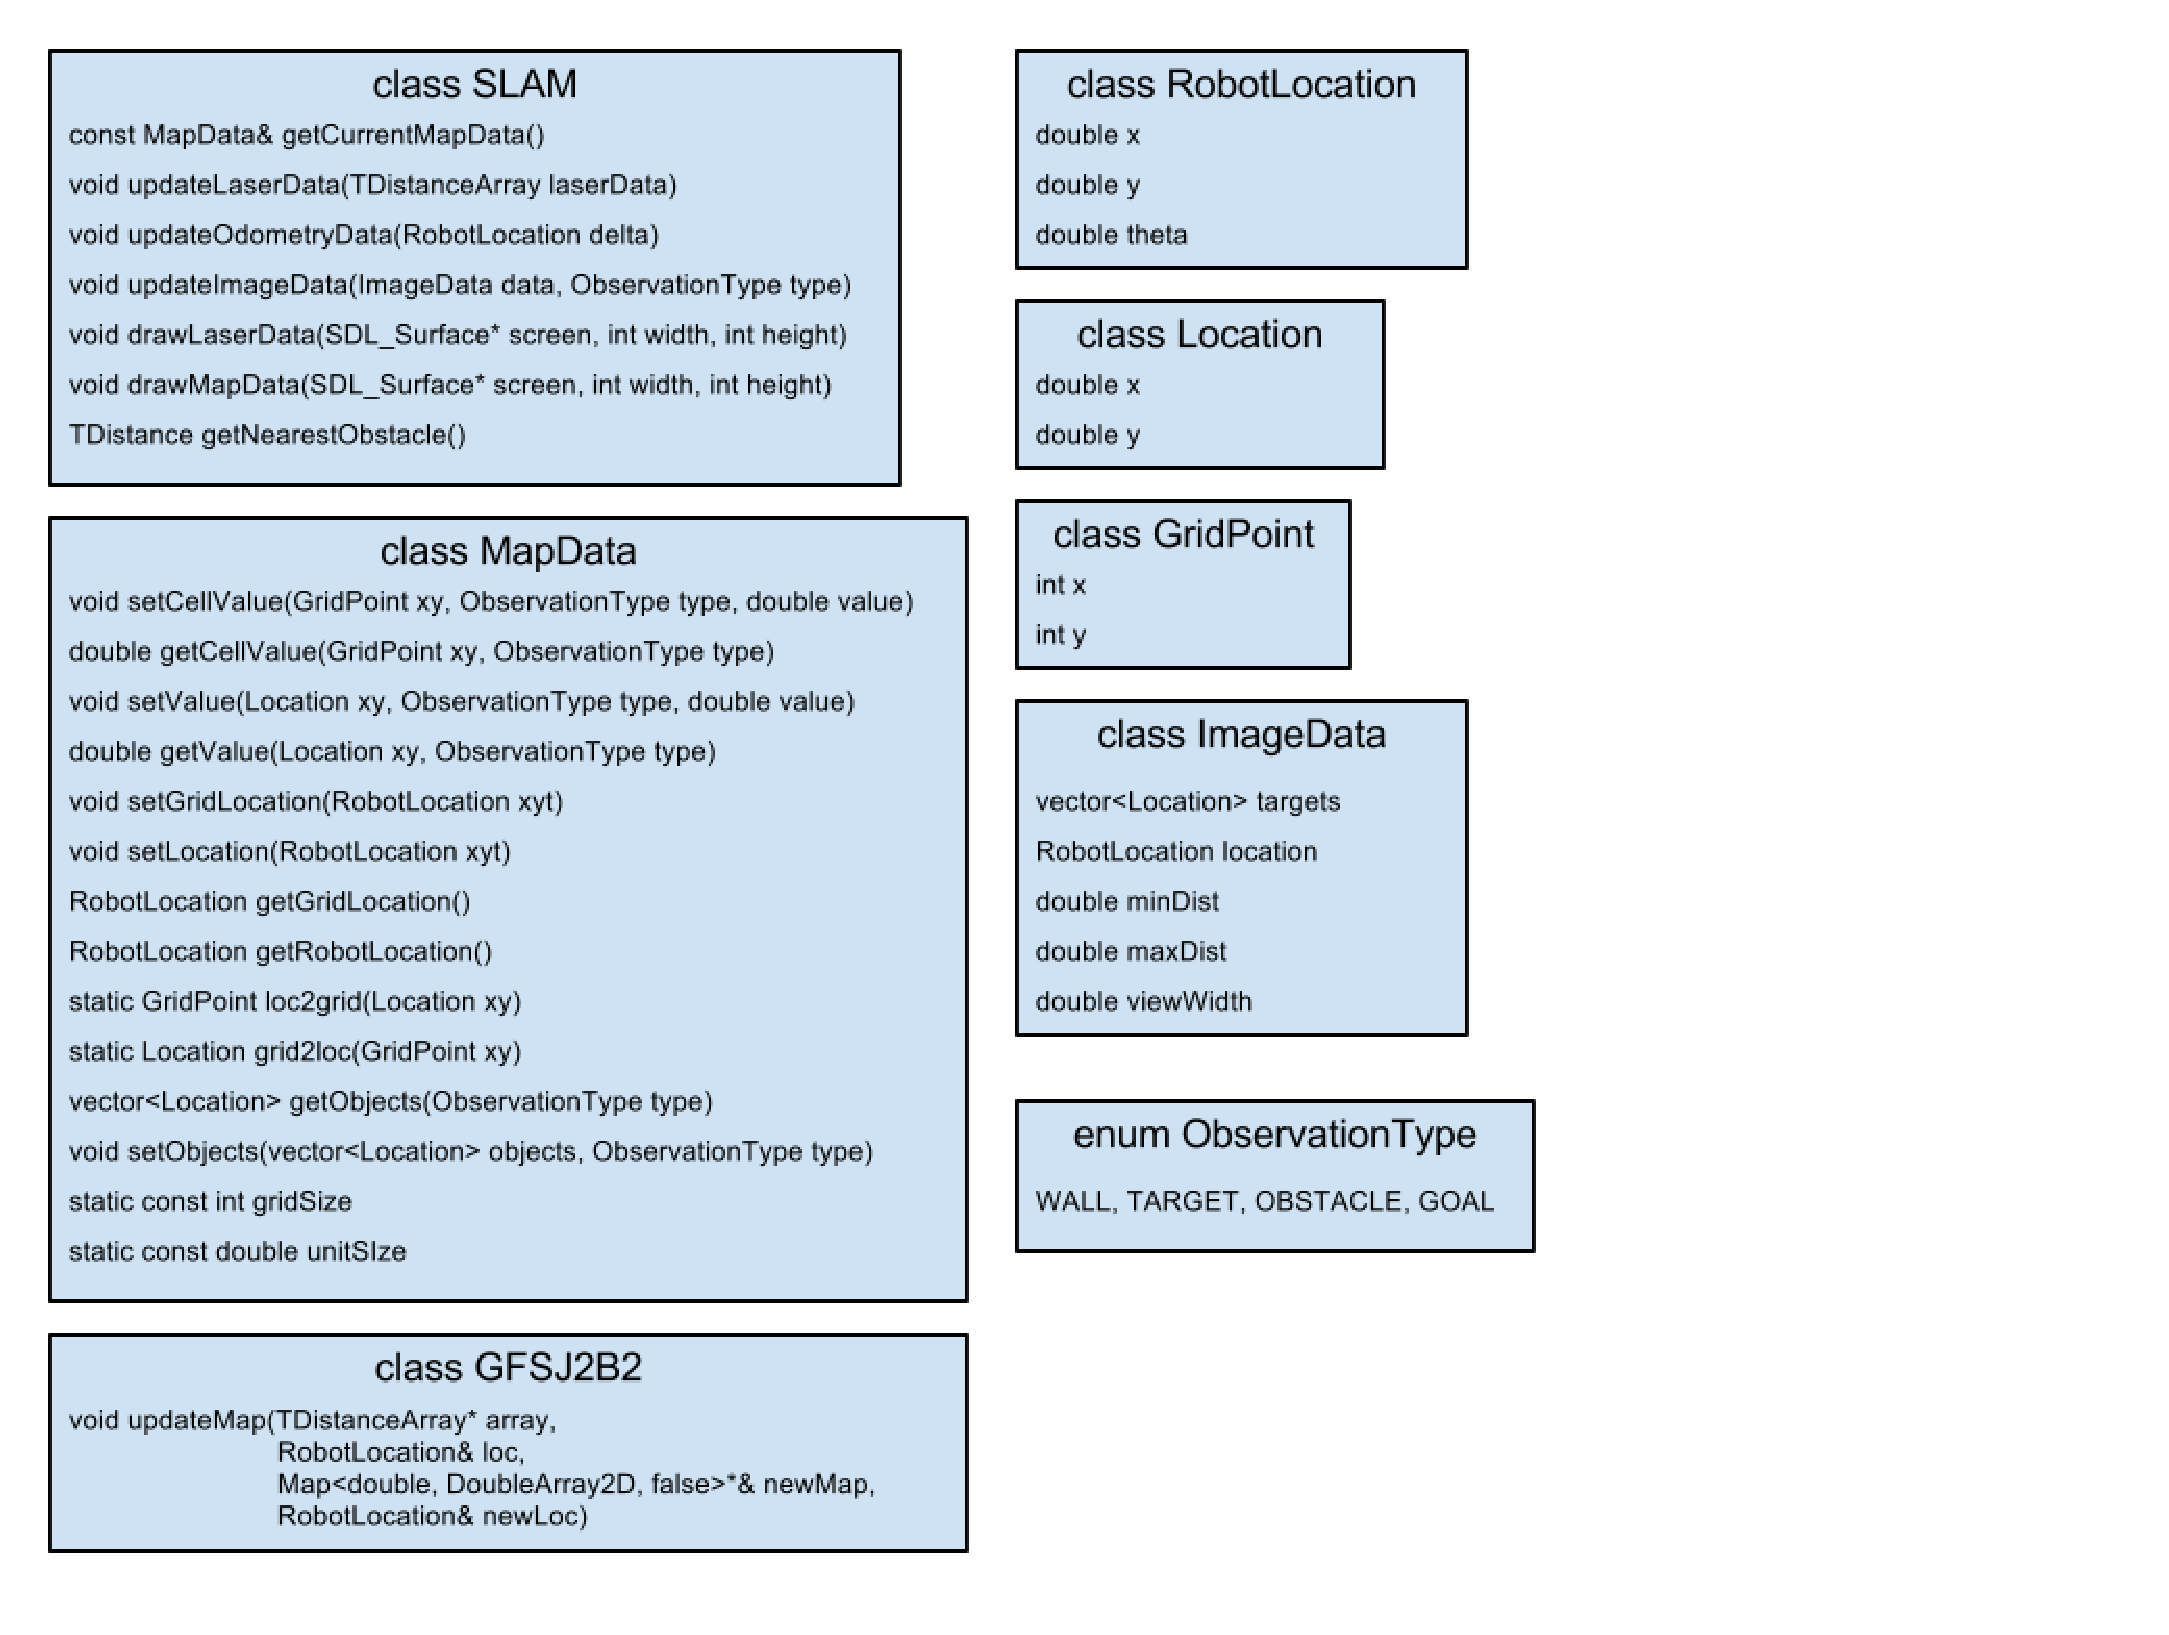
\includegraphics[width=16.0cm]{slam_1.eps}
\caption{Simplified class diagram of the SLAM module}
\label{slam_classes} % The label for the figure. You can refer to the figure by \ref{fig:1} in the text. 
\end{center}
\end{figure}

\subsubsection{SLAM Class}

The SLAM class is the main interface and management class of the SLAM module. The purpose of the SLAM class is to receive data from other modules, perform required preprocessing, send the data in correct form to the gmapping wrapper class (GFSJ2B2), receive map and location updates in return, perform required post-processing and finally make the data available for all the other modules. This class is also responsible for offering the SLAM data visualization service. The data is received via three update methods: updateLaserData, updateOdometryData and updateImageData. 

%The algorithms used in these modules are elaborated in the next subsection.

UpdateLaserData method receives current laser measurement arrays, pairs them with the most recent location estimate and sends them to the gmapping wrapper class. As the gmapping algorithm runs the SLAM update only when the robot has moven a certain amount from the last position, this method will do nothing if the update is not run. When the update is run, however, this method is responsible for extracting the relevant data from the received map and updating the wall information in the current map based on this data. This method is also responsible for keeping the initial location of the robot marked as a goal section in the map and making sure that no walls are marked near the goal. This is done to make sure that the robot always has a goal position that can be navigated to.

UpdateOdometryData method receives odometry updates and integrates them with the current location, thus forming the location estimate between SLAM updates.

UpdateImageData method receives recent image data from the camera module and integrates that data with the existing one. The ImageData object contains a list of parsed targets of certain type, and the parameters of the approximate area that was seen by the camera. The targets that are tracked are via camera are objects (red balls), obstacles (green balls) and goal area (corner points of a blue square).

DrawLaserData method visualizes the latest laser data on the screen in relative coordinates centered on the robot. An example of this can be seen in figure \ref{slam_laser_data}.

DrawMapData method visualizes the current map data on the screen. The data consists of four maps, each presenting certain types of mapped objects, as well as the location of the robot relative to the map. The maps are 2D occupancy grid maps for walls, targets, obstacles and goal area, and each of these is visualized in different color for clarity. An example of these maps can be seen in figure \ref{slam_laser_data}.

\begin{figure}[h]	% Use here 'h' for 'here', 't' for 'top' or 'b' for bottom. '!' makes the figure float.
\begin{center}
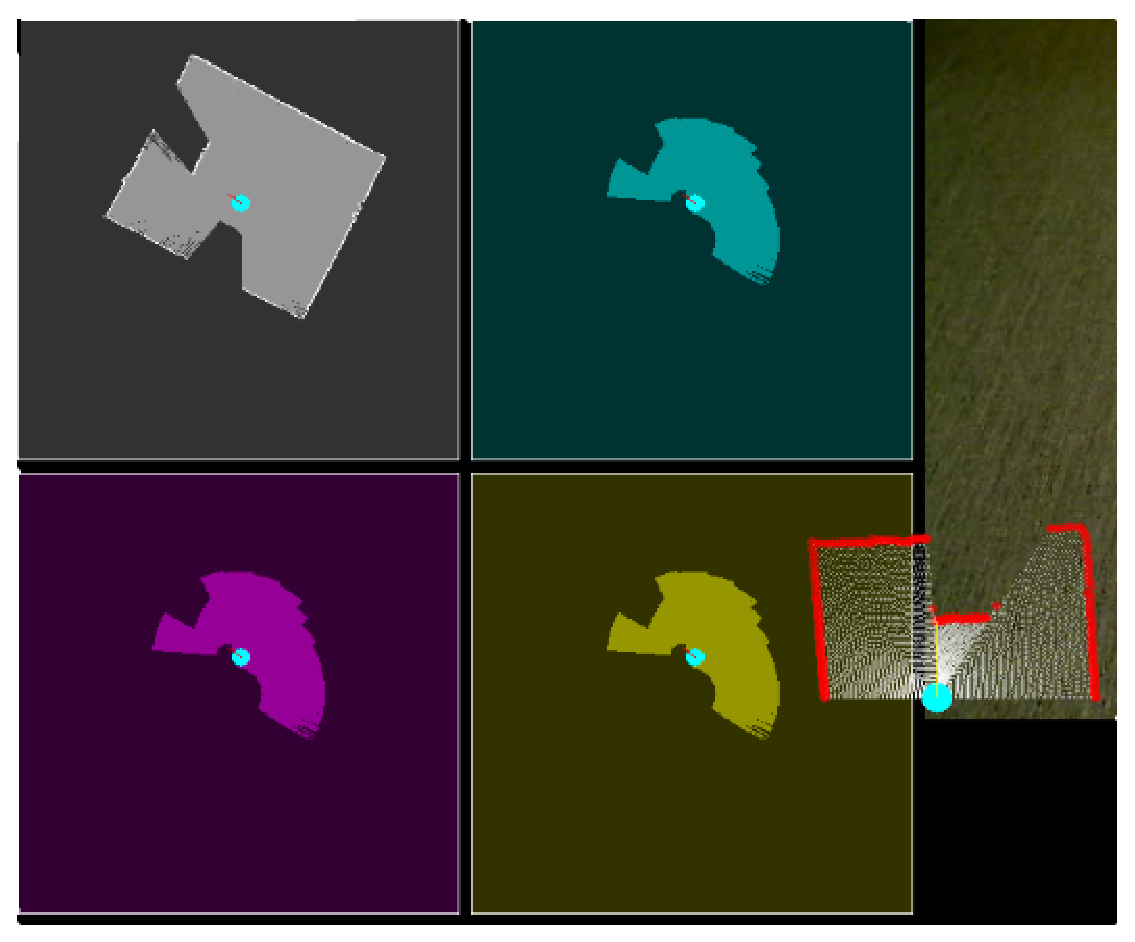
\includegraphics[width=10.0cm]{slam_0.eps}
\caption{The visualized layers of the occupancy grid for different types of objects (from up left: walls, targets, obstacles, goal area), as well as the visualized latest laser measurement (right center). Sadly, this is an older image, but a newer one was not available at this moment.}
\label{slam_laser_data} % The label for the figure. You can refer to the figure by \ref{fig:1} in the text. 
\end{center}
\end{figure}

getNearestObstacle is a short-cut method that simply returns the distance to the closest object that was observed in the latest laser scan measurement (i.e. the minimum measurement in the measurement array).

\subsubsection{MapData Class}

The purpose of the MapData class is to contain all the relevant information of the surroundings of the robot in a 2D occupancy grid form. The class contains an occupancy grid for each type of measurement (walls, targets, obstacles and goal area) and the latest location of the robot in map coordinates (x, y, theta). All the maps are aligned in the same way, so that the robot’s initial location is (0,0,0) and that it is in the center of the map. Thus a grid point with certain index (x, y) refers to the same location in the world in all the maps. It could be said that the different maps represent semantically different objects in a common coordinate system.

The occupancy grid point values usually take values -1 (unexplored cell) or 0..1 (probability of certain type of object existing in this location). However, with objects other than walls, only values 0 and 1 are used. The map values can be accessed either based on grid index (methods setCellValue, getCellValue) or location in the SI-unit coordinates (methods setValue, getValue). The location of the robot can be accessed similarly in grid index coordinates (methods setGridLocation, getGridLocation) or SI-unit coordinates (methods setLocation, getRobotLocation). The difference in these coordinates is, that grid index coordinates are in positive integers and have the origo in the corner of the map, and are mainly used by some internal routines of this module, whereas SI-unit coordinates are in meters from the center of the map, and are used mainly by all other modules.

The targets tracked by the camera are stored also in a list form, as it is much more convenient to use than the occupancy grid form (even though essentially they both carry the same information). For example, it is possible for some other module to request a list of all the target positions for deciding where to go next. The list is a vector of locations of the objects in SI-unit coordinates. The lists can be accessed using methods getObjects and setObjects, although the method setObjects should only be used by certain routines of the SLAM module.

The size of the map grid, gridSize (i.e. how many cells are there in the map in x and y dimensions), and the size of a cell, unitSize (i.e. how large is one cell in x and y dimensions in SI-units), are also publicly available for different uses.

\subsubsection{GFSJ2B2 Class}

The purpose of this class is to act as a wrapper for the gmapping algorithm library. The class has only a single method, which initializes the algorithm, pre-processes the laser scan and odometry data into the required form, calls the library methods and does relevant post-processing if the algorithm performs a SLAM update. (The name of this class comes from Grid Fast Slam wrapper for J2B2.)

\subsubsection{Other Classes}

The module also has other classes, which exist mainly for the purpose of data encapsulation.

RobotLocation class is designed to encapsulate the location of the robot, meaning the x and y coordinates in some coordinate system, as well as the direction the robot is facing, theta, given in radians.

Location and GridPoint classes are designed to encapsulate location information, either in SI-unit coordinates (Location class) or in grid index coordinates (GridPoint class).

ImageData class is designed to be an interface class between the camera and SLAM modules. The object contains a list of objects of certain type identified by the camera module, as well as the approximate area that was seen by the camera, given as a sector limited by two circles (radii minDist and maxDist) and a field of view angle (viewWidth). This is illustrated in figure \ref{slam_image_data}.

\begin{figure}[h]	% Use here 'h' for 'here', 't' for 'top' or 'b' for bottom. '!' makes the figure float.
\begin{center}
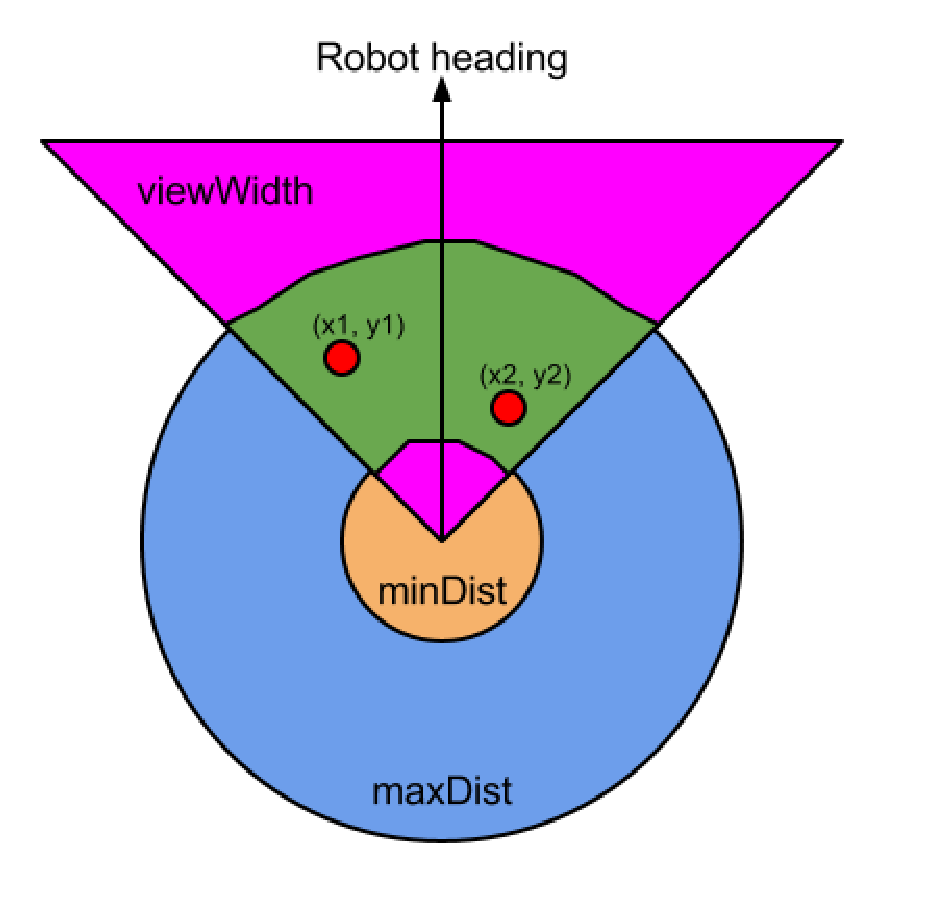
\includegraphics[width=8.0cm]{slam_2.eps}
\caption{Illustration of the contents of the ImageData object. MinDist represents the minimum and maxDist the maximum distance seen. viewWidth represents the total view width (in radians), which is distributed evenly on both sides of the "front axis" of the robot (determined by the heading). The ImageData object contains a list of all the relevant objects that the camera module has identified in the image.}
\label{slam_image_data} % The label for the figure. You can refer to the figure by \ref{fig:1} in the text. 
\end{center}
\end{figure}

ObservationType is not a class, but an enumeration that is defined inside the MapData class. This enumeration is used to determine the relevant type of observation in different cases.

\subsubsection{Module as a Whole}

To use the module, an instance of SLAM class is first created. This will also initialize an empty MapData object as well as the gmapping algorithm. When the first laser measurement is received, and always after the robot has moved a certain amount from the last update, the gmapping algorithm creates updates to the SLAM map, which is then made available to other modules. Between these updates, the location of the robot is approximated by integrating the received odometry data. The target, obstacle and goal area data is updated every time an update from the camera module is received. The latest laser range measurement and the contents of the MapData object are visualized every as often as requested.

\subsection{Gmapping in a Nutshell}

Gmapping is a publicly available implementation of the Rao-Blackwellian particle filter for grid maps \cite{Grisetti_improved}. This subsection shortly describes the main idea behind this method based on this article.

The SLAM problem is to approximate the combined probability distribution of the robot's trajectory ($x_{1:t}$) and the map of the surroundings ($m$), based on past odometry ($u_{1:t-1}$) and laser ranging measurements ($z_{1:t}$):

\begin{equation*}
p(x_{1:t}, m | z_{1:t}, u_{1:t-1})
\end{equation*}

If it would be possible to somehow calculate this distribution, the best estimate for the trajectory of the robot (localization) and the map (mapping) would be the ($x_{1:t}$, $m$) pair corresponding to the maximum of this distribution.

The Rao-Blackwellized particle filter assumes that this problem can be factorized into two separate problems so that the map and the trajectory can be tracked separately:

\begin{equation*}
p(x_{1:t}, m | z_{1:t}, u_{1:t-1}) = p(m | x_{1:t}, z_{1:t})*p(x_{1:t} | z_{1:t}, u_{1:t-1})
\end{equation*}

This factorization allows fast computation, as $p(m | x_{1:t}, z_{1:t})$ can be computed analytically as a map based on measurements from known poses. On the other hand, to compute $p(x_{1:t} | z_{1:t}, u_{1:t-1})$ one can use a particle filter where each particle represents a possible trajectory of the robot. This means that each trajectory has a corresponding map that is calculated based on that precise trajectory.

The particle filter is a discrete approximation of the actual continuous distribution. The gmapping filter consists of a finite number of particles $\{ x_t^{(i)} \} $, that each correspond to one possible trajectory $x_{1:t}^i$. Every timestep when new information is received, the algorithm does the following steps for each particle:

\begin{enumerate}
\item The current position estimate is the last position estimate added with the odometry movement estimate: $x_{t+1}^i=f_1(x_t^i, u_t)$

\item The estimate is improved by scan-matching. This means that the position near the current position estimate which makes the laser measurements fit best to the map is chosen as the new current position estimate: $x_{t+1}^i=f_2(x_{t+1}^i, m_t^i, z_{t+1})$

\item The probability distribution around the current position is estimated by sampling: $p(x)=f_3(x_{t+1}^i, x, m_t^i, u_t, z_{t+1})$. The mean ($\mu_{t+1}^i$) and covariance ($\sigma_{t+1}^i$) of this sampled distribution are also calculated. The weight of the particle is calculated based on the integral of the sampled distribution: $w_i=\Sigma[p(x)]$

\item The current position estimate is replaced by one drawn randomly from a Gaussian distribution with mean and covariance as calculated in last step: $x_{t+1}^i$  drawn randomly from  $N(\mu_{t+1}^i, \sigma_{t+1}^i)$

\item The map is updated based on the current position estimate and the laser measurements: $m_t^i=f_4(x_{t+1}^i, z_{t+1})$
\end{enumerate}

When the probabilities of the particles become too "peaked", meaning that there are many particles with very small weights, a re-sampling is performed, where a large number of new particles are generated based on the existing ones, after which the ones with smallest weights are removed with the largest probability. This generally increases the amount of good estimates while still keeping the amount of particles the same.

The filter updates are however only done after the robot has moved over a certain distance from the last location, as the updates require a considerable amount of time and as odometry data should be sufficiently accurate for very short distances. After each filter update, the particle with the largest weight can be used as the current best estimate of the trajectory of the robot and the map of the surroundings.

\section{Navigation}

The main planner orders the navigation module to find a route to a wanted destination. This route is then handed out to the motion controller. Navigation consists of a path finding algorithm working on a grid (MapData from SLAM), and some pre-processing functions to make the occupancy grid data fit better for the algorithm.

The path finding algorithm was developed separately at first, with a bigger grid and a separate visualization program, which can be seen in figure \ref{navi_first_path}.

\begin{figure}[h]	% Use here 'h' for 'here', 't' for 'top' or 'b' for bottom. '!' makes the figure float.
\begin{center}
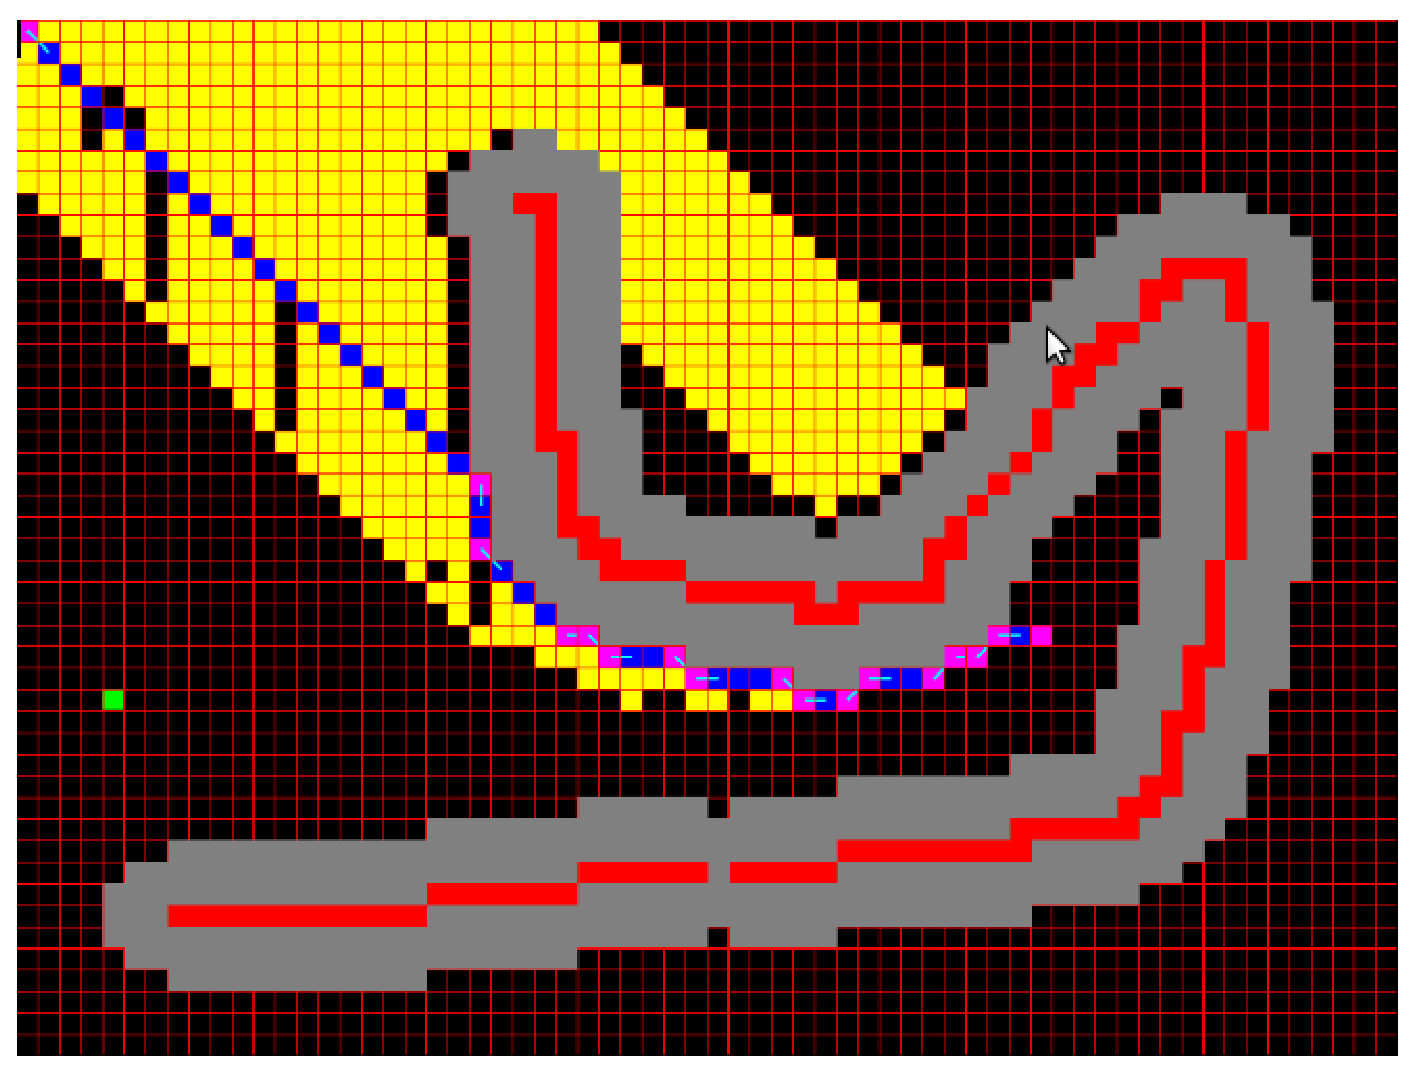
\includegraphics[width=10.0cm]{navi_1.eps}
\caption{A toy program for testing out the path finding code. Red: walls, grey: virtual obstacles generated by dilation, blue: final route, purple: route's corner points, yellow: other areas investigated by the search.}
\label{navi_first_path} % The label for the figure. You can refer to the figure by \ref{fig:1} in the text. 
\end{center}
\end{figure}

\subsection{Path Finding}

The path search works with the A* algorithm \cite{hart1968formal}. A* is an extended Dijkstra’s search, based on a heuristic value of current estimate to the goal.

The algorithm's inputs are the source and destination nodes and the current world map (2d occupancy grid, pre-filtered as described in section \ref{navi_prepros}). It outputs a list of grid vertices that form a safe, connected path from source to destination.

Because the used A* library (boost::graph \cite{navi_boost})  works on a graph, the world map (a simple two-dimensional array, which is not a graph as described by the library) is used with a wrapper to generate vertices (grid points) and virtual edges (vertex-vertex connections) for the algorithm based on the map information. Vertices map 1:1 to free-space (traversable) grid points (they just carry additional information on the graph for implementation-specific details in the library), and edges are generated so that from each vertex there exists an edge to every surrounding 8-neighbour. The edges' weights are set to match relative physical distances between vertices: axis-aligned edges have length 1, and diagonal edges have length $\sqrt{2}$.

Due to the nature of graph searching, if the navigator is asked to find an impossible route, it visits each node in the whole graph. Only after that it is sure that no possible route exists.

In retrospect, it would have been easier to just implement the A* search by ourselves, because the boost library is quite complicated. There was not a direct support for implicit grid-based graphs. The library is very flexible, though, and any required changes during development were relatively easy to fix when needed.

\subsection{Preprocessing}
\label{navi_prepros}

Plain A* uses just a graph with no information about the robot's physical constraints. That is why the raw data on floor and wall locations must be pre-filtered so that the robot can be assumed to be a single point in the searched graph. This is done very naively by thresholding the probability map with a predetermined constant, and dilating every wall point in the grid by the robot radius plus a safety constant, which generates virtual obstacles around every wall. In this way, we get a simple state-space for the search.

To work around some inaccuracies in SLAM and unknown data in the beginning, the location of the robot is marked as free space; it was noted that without this, the map sometimes contained walls at the robot location, which makes routing obviously impossible because the route starting point usually is at the robot center.

\subsection{Post-processing}

The grid locations of the resulting route are simply translated back to physical locations for the motion control by using the functions supplied by SLAM.

Initially, we planned to use a different algorithm for motion control, and filtered out the points from the navigated list that do not change the robot's heading, i.e. points that do not give new information. The heading directions were also added to the resulting corner points. This was finally not needed, because the motion controller produced very smooth paths anyway, and it filtered nearby points away automatically.

\subsection{Other Uses}

The A* algorithm also keeps track of distances from goal to each visited node. This information is used to find the nearest target to pick up, and also to go to the farthest point from the robot location.

\subsection{Architecture}

The path finding algorithm itself is just included as an utility tool, and it doesn't need to understand anything robot-related and it doesn't depend on other modules. The navigation module keeps track of the current map and robot location, though; each time the SLAM updates its map, navigation's map structure is updated via the main program. This map information is held inside the navigator and used when other modules ask about best routes, farthest points, route lengths, and so.

As said, the boost path finding utility needs quite complicated wrappers to work on a grid. The utility files include classes for internal use: grid vertices and edges, an abstraction for a grid container, and much iterators, getters, traits, and template specializations for the boost algorithms. The graph search enumerates adjacent vertices for each vertex to find out where to search further, and uses a visitor function for each examined vertex to check if the goal vertex has been found. Internally, the boost astar search is implemented as a specialized breadth first algortihm.

\subsection{Discussion}

The A* might not be the best algorithm for this task as-is.

At least some coefficient for near-wall positions could have helped from crashing to some walls because of physical inaccuracies. It would be good if the robot would prefer driving farther away from walls by default. The edge lengths for vertices near walls could be virtually enlarged, to give the algorithm some penalty in critical locations but still to make it able to go near the obstacles if needed. Originally the edge lengths map to physical distances, but the algorithm does not care, and that measure is not really needed. Currently, the algorithm finds optimal paths, based on the assumption that the robot can only work on a grid.

Some optimization for more smooth paths could have been used. The robot is not exactly walking in a grid, but in a real world, so that sub-gridpoint locations are possible. The algorithm assumes that only available locations are discrete points on the grid.  Theta* \cite{nash1999theta}, "any-angle path planning", is one such optimization. In figure \ref{navi_debug_user}, it can be clearly seen that a more straight path is possible, but it involves walking at a better precision than the map size.

\begin{figure}[h]	% Use here 'h' for 'here', 't' for 'top' or 'b' for bottom. '!' makes the figure float.
\begin{center}
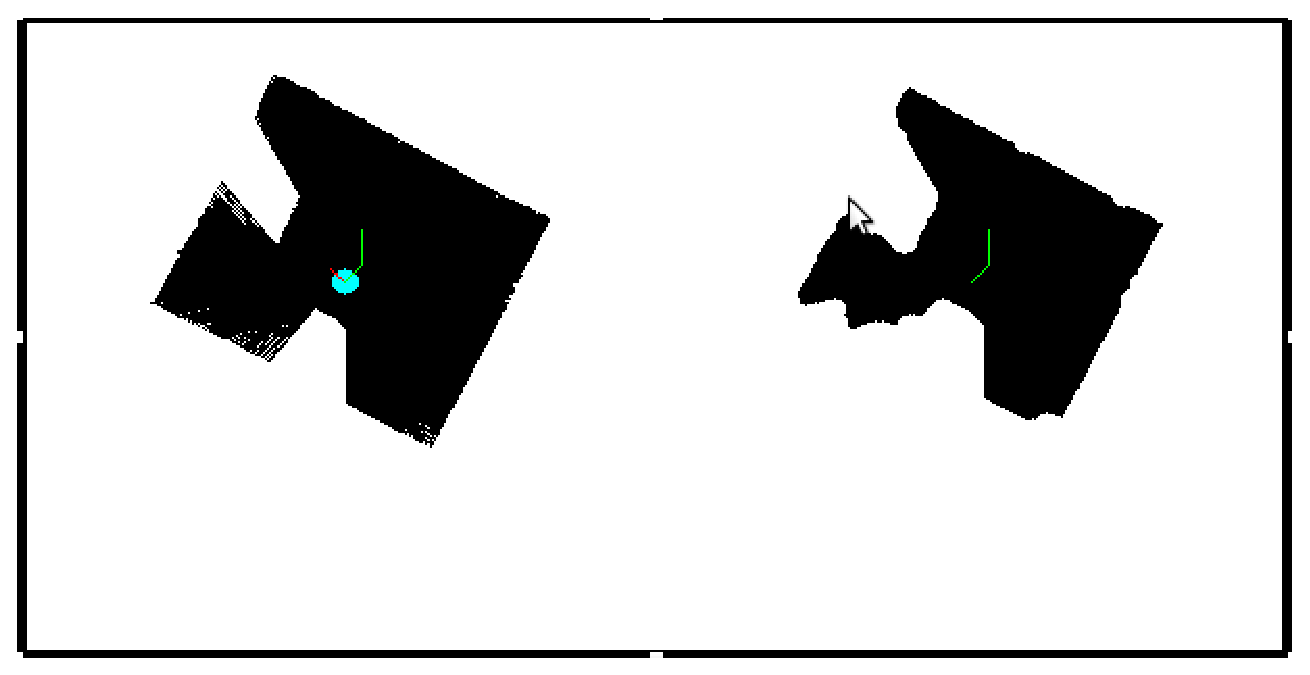
\includegraphics[width=10.0cm]{navi_2.eps}
\caption{Debug/information view in the user interface for the navigation module. On the left: thresholded occupancy grid. On the right: dilated search map. The green line is the navigated route, and the cyan circle represents the robot.}
\label{navi_debug_user} % The label for the figure. You can refer to the figure by \ref{fig:1} in the text. 
\end{center}
\end{figure}

\section{Motion Control}

\subsection{Introduction}

This module is in charge of the robot's movement. It sends information on the desired velocity and angular speed to the built-in robot controller and gets back information on their current state. The module gets the robot's current location from main planner when the main planner asks motion control to move to the target location. The navigation module gives this information as pre-defined waypoints towards the target location, which are saved (and updated during the task) in the waypoint list that the motion control reads. When the robot has gone through the route it has been given, motion control makes the robot stop and waits for a new list of waypoints to a target location. When it gets it, it turns to the orientation of the first waypoint before moving forward.

In addition to robot movement control, the motion control module contains the control of the servo movement. These servos include the camera servo and the servo to move the hatch manipulator. Both can be asked to return their current position and be given a new desired position. 

\subsection{Module Architecture}

The Motion control module, in short Motion, is divided into two classes. The first of these, MotionControl class, contains all the methods needed to move the robot to the desired direction in correct speed. The second, ServoControl class, is in charge of controlling the camera and hatch servos. This class is further described in Object recognition section \ref{servo}. Next, we will give a little more detailed look on Motion control module's classes.

\subsubsection{MotionControl Class}

In the class MotionControl, a method called iterate takes care of the main functionality of moving the robot. It controls the robot's angular direction and calculates the route between its current position and the next waypoint location as Euclidean distance. It also calculates the error between its current angle and the angle of the straight line to the target waypoint. It then uses a slightly modified P-controller to see that it holds this route: angular speed is controlled with P term and the velocity is changed so that the robot slows down when the angular error increases.

Other methods used in the MotionControl class are, among other things, responsible for telling the robot controller the desired speed and refreshing this information as well as managing the waypoint list gotten from the navigation module. The robot can be stopped with a specific method, and also the robot's behavior at the end of the mission is regulated, as the robot is told to back off at the goal area to leave the targets and then move once back and forth to ensure that all the targets are within the goal area.

\subsubsection{ServoControl Class}

ServoControl class contains a few small methods for moving all the servos. The hatch servo can only be moved up and down, and also the camera servo is fixed to hold a forward facing.

\section{Object Recognition}

\subsection{Introduction}

The purpose of the Object recognition (or more familiarly Camera module) is simply to detect targets and the goal area. Because of the nature of the open manipulator of the robot, we decided also to track non-targets, with an effort to avoid picking them.

The camera on the robot was a simple webcam mounted with two servos on the top of the robot. Two servos made it possible to rotate the camera with tilt and pan angles. For simplicity, we decided to use just two pre-defined angles for tilt servo and leave the pan servo on its center position. There were no limits in our code to use both servos, transformations from camera coordinates to robot coordinates should be correct anyway.

\subsection{Module Architecture}

The module consists of one main class Camera and two helper classes Camutil and CameraCalibration. There is also additional ServoControl class in motion control module, just for controlling camera servos. Camera calibration class was tested and found that it was working. Although it was used for a while, we left the calibration apart from our final solution, as the camera's original calibration was good enough.

\subsubsection{Camera Class}

Camera class is the main class of the Object recognition module. The class contains methods to communicate with actual webcam, fetch the current image from the camera, and offer image data for J2B2's main program to be drawn on a screen. The class has also interfaces to move camera to predefined positions, check the camera calibration and to update processed camera data for SLAM.

Camera module stores last image in cameradata struct, as well as servo positions and a location of the robot where the image is taken. It stores also last calculated target locations in a real world coordinate system.

The most difficult part of the Camera module is in the updatePositionOfTargets method where objects that are detected from camera image are transformed into the real world coordinates. To do that process we are using Eigen library that is a linear algebra library for C++.

Using predefined parameters for camera (focal length 3.7 mm, experimentally hacked physical pixel size on image sensors 0.07 mm, camera tilt angle fix 0.07 rad, and camera position in robot coordinates (0, 0.72, -0.27)) we are able to construct rotation matrices for robot and camera angles and finally transformation matrices for each detected object.

\begin{verbatim}
Vector3f P_cam(0, 0.72, -0.27);
Vector3f P_rob(robotloc.y, 0, -robotloc.x);
Matrix3f R_cam(rotx(theta_cam));
Matrix3f R_rob(roty(theta_rob));
Vector3f p(ball.x, ball.y, 1);
Vector3f v = R_rob * R_cam * Ki * p;
double l = -P_cam(1) / v(1);
Vector3f P0 = P_rob + R_rob * P_cam;
Vector3f P = P0 + l * v;
Vector3f t(-P(2), P(0), 0);

P_cam     the position of the camera in real world coordinates
P_rob     position of the robot in real world coordinates
R_cam     camera servo position (tilt angle)
R_rob     robot angle in real world coordinates
p         object on the image plane
Ki        camera internal matrix containing e.g. focal length and image size
v         direction vector from camera to target
l         distance to ground level along vector v from camera origo
t         final coordinates of the object in a real world coordinate system
\end{verbatim}

The theory of the pinhole camera model is adapted from multiple sources, for instance from \cite{pinhole_cam}.

\subsubsection{Camutil Class}

Camutil class was intended to be a class containing some utilities for Camera module. In fact it contains the most central methods to detect object positions in a camera image and transform coordinates into the real world.

All image processing is made with OpenCV camera library. First image is converted from MaCI::Image::CImageContainer to OpenCV's Mat format and from BGR to RGB color space. When finding objects from the image, it is converted again from RGB to HSV format and then using pre-defined color areas for targets, non-targets and goal area, image is converted to binary color image.

Now, having separate images for targets, non-targets and goal area, images are going to be filtered using two pixel dilation. Dilation cleans the image and removes single and separate pixels. After that we are using OpenCV's findContours method to find connected contours from binary image. Contours are filtered based on their size, so that all round shaped contours with radius less than 13 pixels are filtered out. Also, all contours whose area is smaller than half of the area of a full-sized round object with the detected radius, are excluded.

For detecting the goal area the methods are mostly the same, but instead of finding circular objects, we are looking for a rectangle with an area between hat-constants 10000 and 640*480/2 pixels.

\subsubsection{CameraCalibration Class}

As mentioned before, CameraCalibration class contains working methods to calculate internal parameters for any camera. Calibration uses multiplied images or short video sequences where check board is in view. It uses ready made method findChessboardCorners provided by OpenCV to detect chess board and finally calculates internal parameters and distance coefficients by calling OpenCV's calibrateCamera method.

\subsubsection{ServoControl Class}
\label{servo}

ServoControl class is a container that stores information about servo positions. It also scales servo control parameters from [-pi, pi] to [-1, 1].

\section{Manipulator}

The manipulator consists of a recycled cardboard around the robot's floor contact level. The cardboard is fastened to pre-existing holes with six shortened prototype screws and compatible nuts. The robot with the manipulator and its fastening mechanism are shown in figures \ref{j2b2} and \ref{screws}.

\begin{figure}[h]	% Use here 'h' for 'here', 't' for 'top' or 'b' for bottom. '!' makes the figure float.
\begin{center}
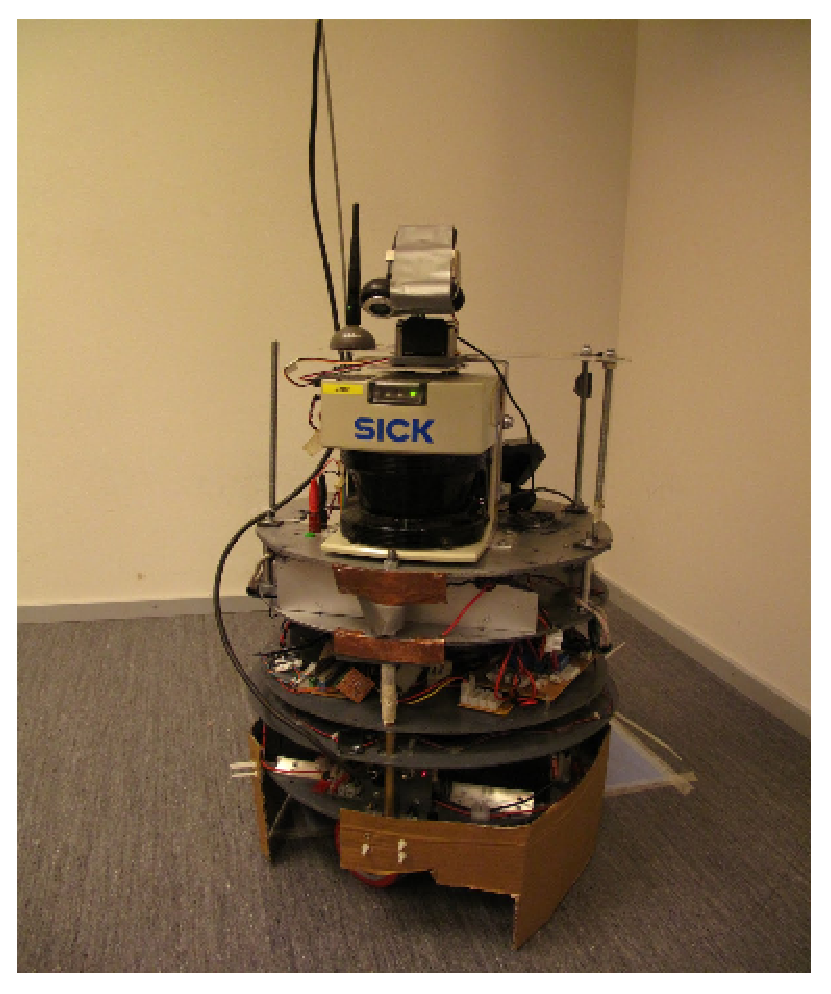
\includegraphics[width=8.0cm]{j2b2.eps}
\caption{J2B2 robot with its manipulator, the cardboard skirt.}
\label{j2b2} % The label for the figure. You can refer to the figure by \ref{fig:1} in the text. 
\end{center}
\end{figure}

\begin{figure}[!]	% Use here 'h' for 'here', 't' for 'top' or 'b' for bottom. '!' makes the figure float.
\begin{center}
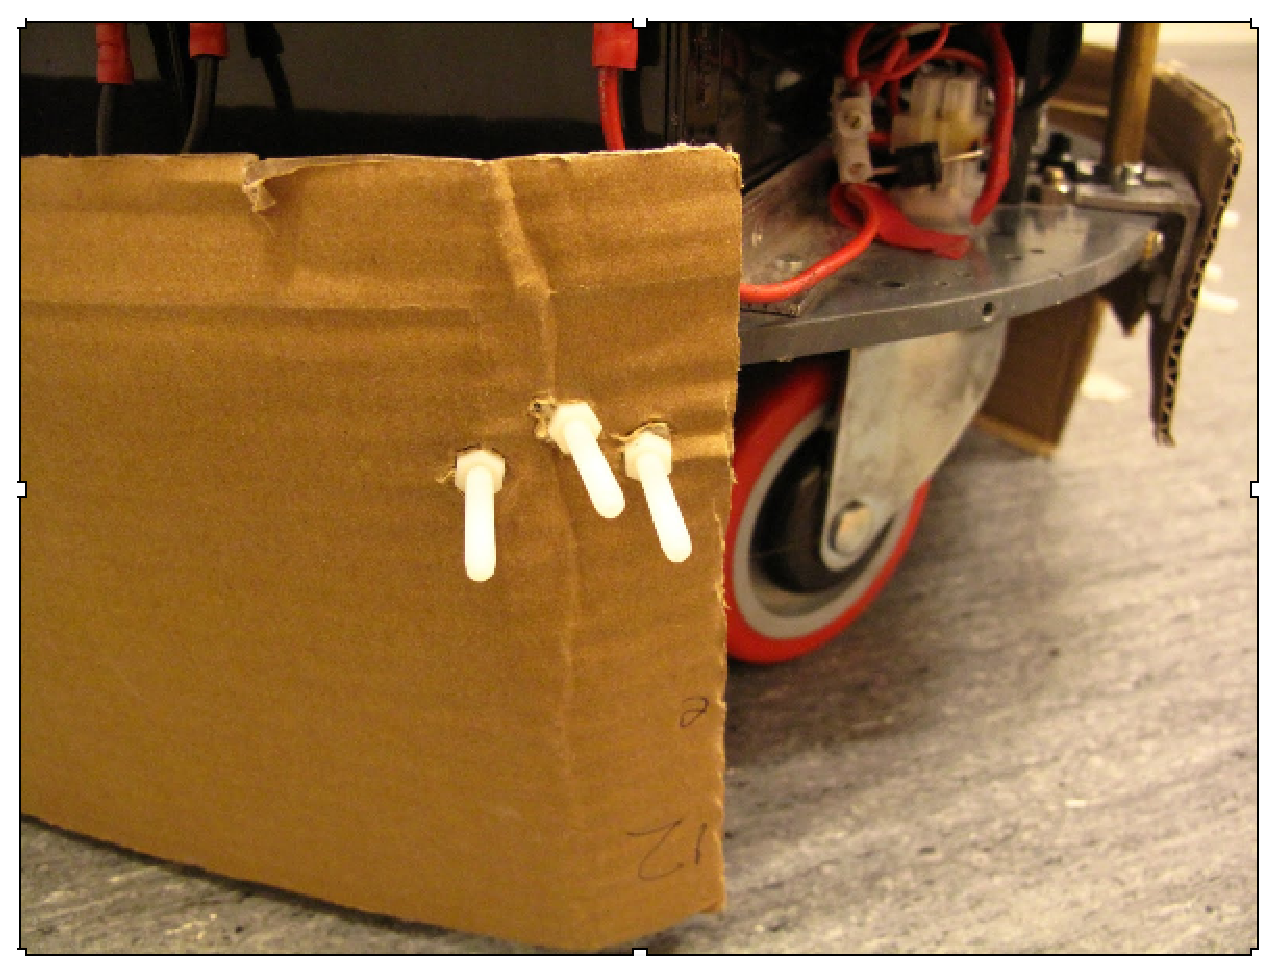
\includegraphics[width=8.0cm]{screws.eps}
\caption{The fastening mechanism of the cardboard manipulator: six prototype screws and compatible nuts.}
\label{screws} % The label for the figure. You can refer to the figure by \ref{fig:1} in the text. 
\end{center}
\end{figure}

A slight slit in front of the robot is left open to catch targets. The targets are then accumulate below the robot. Being in direct contact with the wheel, several tests are performed to verify that they do not bother the robot when moving and the wheels are free to change direction. This is possible thanks to the low weight of the targets. The purpose of this is to capture all of the objects the robot drove over. This design is made possible to use due to the low friction between the floor and the objects it is to gather.

A snow-plow-like hatch that covered the entry area was a part of the original design of the manipulator. Its purpose was to prevent non-targets from being collected. The hatch was abandoned a few days before the final competition due to possibility of a frontal or rotational collision with the environment, creating a danger of damage to the hatch and the servo. The hatch itself was fashioned out of aluminium, recycled cardboard, prototype screws, a recycled servo and transparent, hard plastic. Holes were drilled into the lowest platform of the robot and the hatch was attached into those using two small screws and nuts. The servo was connected to the same board to which the robot's camera is attached to. The hatch is shown in figure \ref{hatch}.

\begin{figure}[h]	% Use here 'h' for 'here', 't' for 'top' or 'b' for bottom. '!' makes the figure float.
\begin{center}
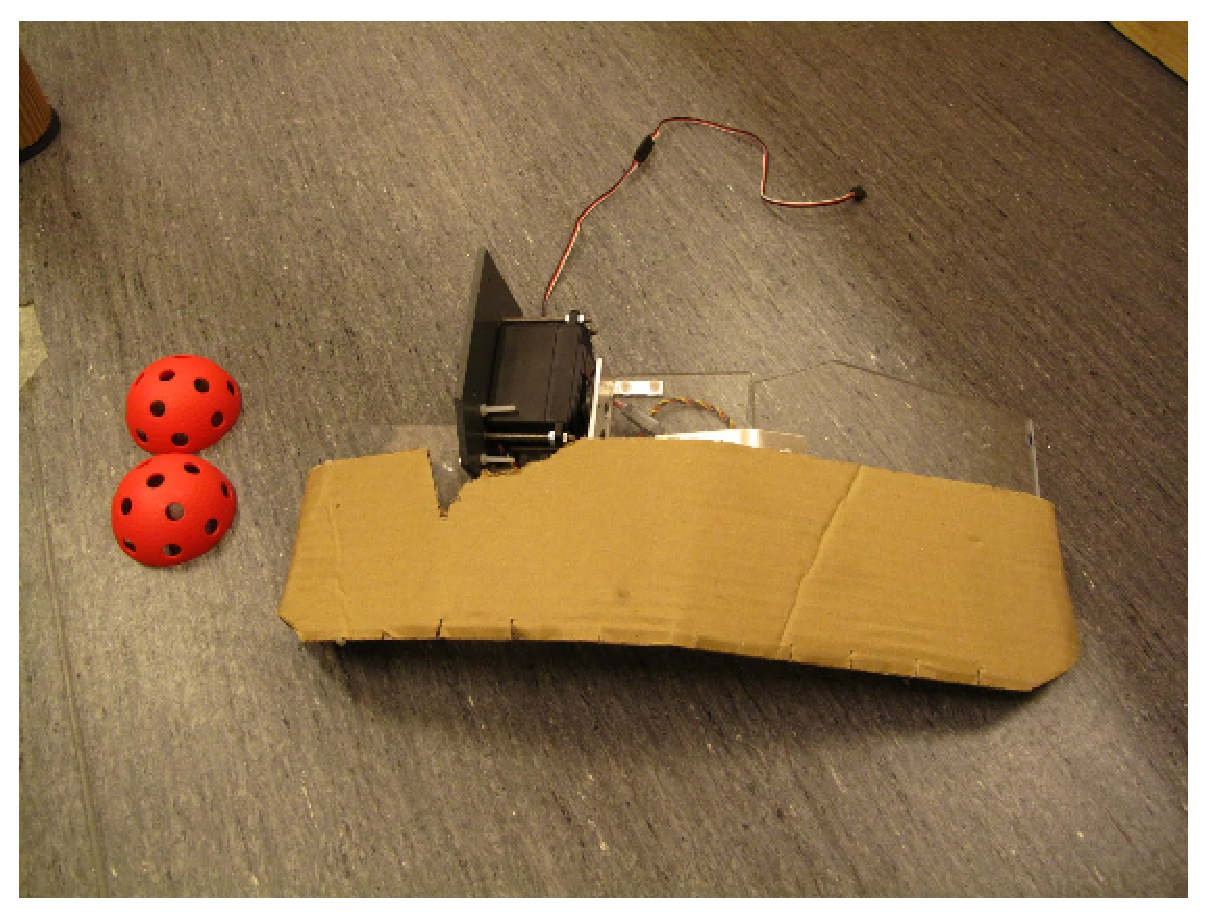
\includegraphics[width=8.0cm]{hatch.eps}
\caption{The manipulator hatch with two targets for scaling.}
\label{hatch} % The label for the figure. You can refer to the figure by \ref{fig:1} in the text. 
\end{center}
\end{figure}

When the initial manipulator design had been completed and agreed as robust, we proceeded to build an experimental, most ambitious design with lower chances of being implemented - a coffee gripper (see e.g. \cite{brown2010universal}). The first coffee gripper consisted of a 12-volt air pump, a plastic tube, a balloon 60 cm in diameter (if inflated, but the balloon was kept in its deflated state), coffee, a piece of a coffee filter and a couple of zip ties. The first balloon proved to be too small to pick up the targets in the competition task, but it worked in picking up smaller objects such as dice and keys. Upgrading to a 90 cm diameter balloon was not sufficient to pick up the task targets either, and the line of development was abandoned at that point due to time constraints and high costs, as balloons of an even greater size could not be found within the budget limits and the time remaining at that point. The coffee gripper prototype with the bigger balloon can be seen in figure \ref{coffee} and the parts of the air pump and its control servos in figure \ref{pump}.

\begin{figure}[h]	% Use here 'h' for 'here', 't' for 'top' or 'b' for bottom. '!' makes the figure float.
\begin{center}
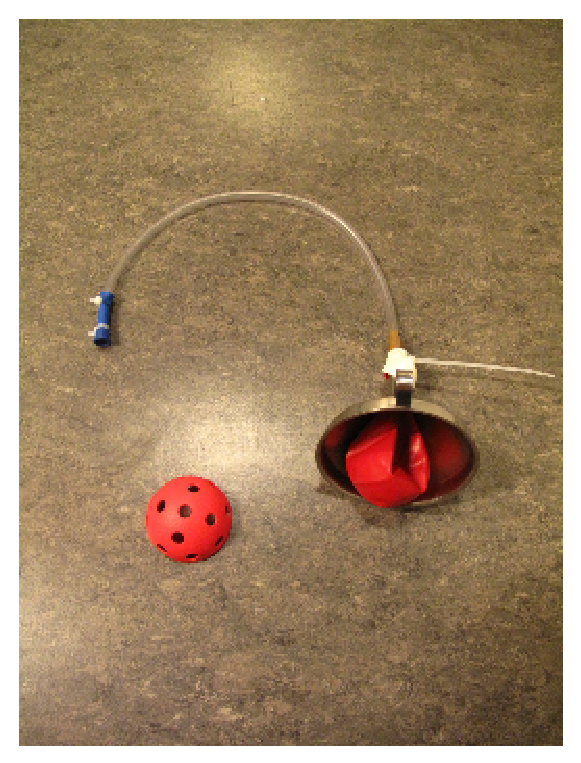
\includegraphics[width=8.0cm]{coffee.eps}
\caption{The prototype of the coffee gripper.}
\label{coffee} % The label for the figure. You can refer to the figure by \ref{fig:1} in the text. 
\end{center}
\end{figure}

\begin{figure}[!]	% Use here 'h' for 'here', 't' for 'top' or 'b' for bottom. '!' makes the figure float.
\begin{center}
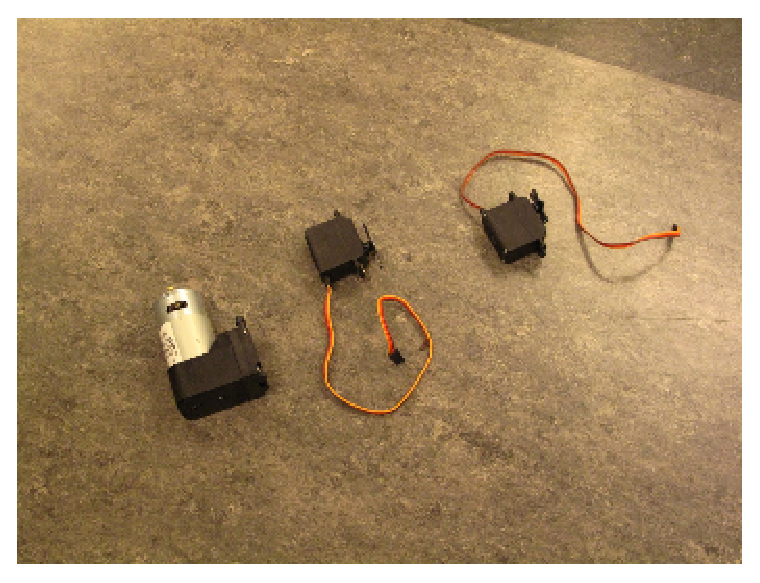
\includegraphics[width=8.0cm]{pump.eps}
\caption{Air pump and servos for the coffee gripper prototype.}
\label{pump} % The label for the figure. You can refer to the figure by \ref{fig:1} in the text. 
\end{center}
\end{figure}

\section{Planner and State Machine}

\begin{figure}[!]	% Use here 'h' for 'here', 't' for 'top' or 'b' for bottom. '!' makes the figure float.
\begin{center}
\includegraphics[width=12.0cm]{fsrfsm.pdf}
\caption{Simplified state machine diagram. Timeout mechanism not visualized.}
\label{fsm} % The label for the figure. You can refer to the figure by \ref{fig:1} in the text. 
\end{center}
\end{figure}

The planner \ref{fsm} is a simple state machine that is implemented mostly as a large switch-case-structure. This is possible because there are not really that many states, the transitions are quite simple, and there was much lack of time because it was the last thing to be done.

In the beginning, the robot rolls a full circle to get a good scan of the surrounding world. Then, it enters an exploration loop to find targets to pick up.

When the robot sees a target, it will calculate the path to all the targets in the task list and choose the shortest path. If the targets can not be reached (e.g. if the robot has not seen the area that it could use for reaching the target) the robot will continue exploring. Otherwise it will enter go-to-target-state.

When the robot is going to the target it will follow the path from navigation until it is close enough the target. Then it will take a closer look at the target by lowering the camera. This is done because the camera measurements done far away have more errors than closer measurements. After the position of the target has been corrected to more accurate one, navigation re-navigates the target and the robot will move onto the target in approach-pick-up-state. It will also move a bit further - if possible without crashing to the walls - to ensure that the target is really inside the container. The the state is pick-up, the camera is moved back up and the counter of the targets is increased by one.

In case the counter tells that all ten targets have been gotten, the state changes to go-return-to-goal, where the robot tries to navigate to the goal, and if if finds this impossible, it will explore a bit more. If the path to the goal is find, the state changes to return-to-goal and robot follows the path to the goal.

When the goal is reached, the robot drives a bit further and then backs off in release-targets-state for releasing the targets. Then it will repeat this behaviour for second time for making the releasing more reliable.

In state machine there is also back-off-state, which is entered if the bumpers are hit. This state will cause the robot to back off until the bumpers are not hit, and then robot will return to explore-state.

If the time for the task is nearly up, meaning that 13 minutes have passed, the state will change to go-return-to-goal-state if it is not already in some of the states where it should be going to the goal for final time.

After the task is finished and the balls are returned, the robot enters end-state, where it says “Hurraa” and the manual control is switched back on.

\section{Results}

On the eve of the final demonstration of the project's results, functional solutions for all the modules of the software have been developed and a functional manipulator has been built. Also the integration of the modules has proven to be successful. However, some more work especially in the integration part would have been useful.

At its current state, the robot is able to map an unknown area and avoid obstacles. It is also able to collect the desired targets, although it has never been fast enough to find and collect them all before the mission time has come to an end and the robot has had to return to the goal area. There have also been problems with the robot’s precision when collecting targets. Sometimes, when coming closer to a target, the robot will turn to a slightly wrong direction due to the caster wheel, and fail to collect a target despite the fact that it thinks it has collected it.

When avoiding walls and other obstacles the robot has been quite successful, but avoiding unwanted targets has not always been as trustworthy. The robot tries to avoid them, but the avoidance manoeuvre has in many cases been too subtle, and the disturbance caused by the caster wheel has resulted in the robot accidentally collecting the unwanted target instead of avoiding it.

In general, the robot has however managed to accomplish the mapping, searching and collecting parts of the mission relatively well, with not much seemingly illogical behaviour. When returning to the goal area and releasing the targets the robot has been on time, but the releasing manoeuvre would need some more fine adjustment. The robot tends to return most of the targets within the goal area, but does not manage as well when trying to push those outside the area inside it. In fact, the robot sometimes pushes the targets it has first successfully returned away from the goal area again.

The problems detected about the robot's behaviour are mostly of the kind that would only need some more testing and fine adjustment. Anything that would be seriously wrong with the logic of the software has not been detected, and the robot is able to acceptably finish its mission.

During the final demonstration, the robot suffered from a demo effect caused by last minute changes in the code the previous night. The changes accidentally caused the robot to calculate its route to unreachable targets multiple times instead of doing it only once and deciding them permanently unreachable. When this problem was fixed, the behaviour was more like what had been seen during testing. Demonstrations on the robot's behaviour can be seen in figures \ref{world} - \ref{success}.

\begin{figure}[h]	% Use here 'h' for 'here', 't' for 'top' or 'b' for bottom. '!' makes the figure float.
\begin{center}
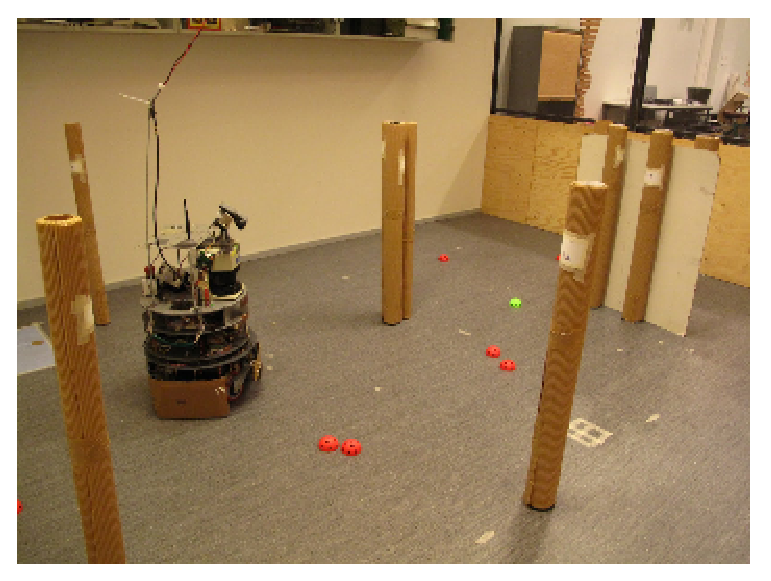
\includegraphics[width=8.0cm]{j2b2_world.eps}
\caption{J2B2 moving around the test environment.}
\label{world} % The label for the figure. You can refer to the figure by \ref{fig:1} in the text. 
\end{center}
\end{figure}

\begin{figure}[!]	% Use here 'h' for 'here', 't' for 'top' or 'b' for bottom. '!' makes the figure float.
\begin{center}
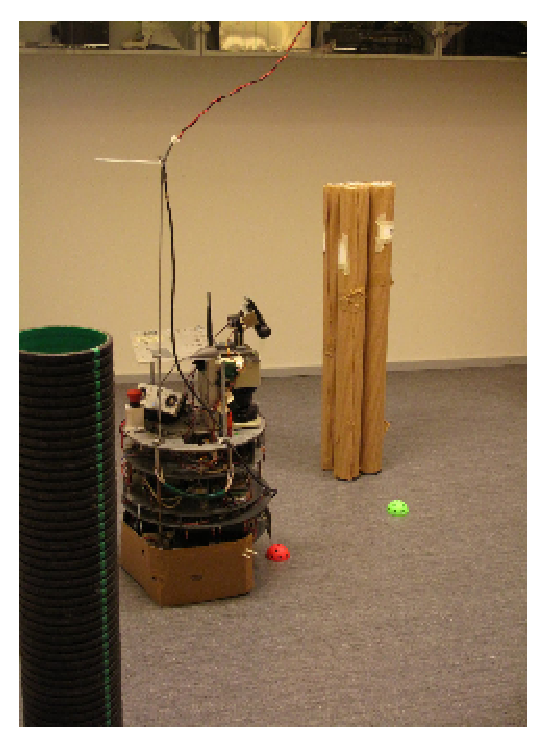
\includegraphics[width=8.0cm]{collect_target.eps}
\caption{J2B2 collecting a target into the cardboard skirt manipulator.}
\label{target} % The label for the figure. You can refer to the figure by \ref{fig:1} in the text. 
\end{center}
\end{figure}

\begin{figure}[!]	% Use here 'h' for 'here', 't' for 'top' or 'b' for bottom. '!' makes the figure float.
\begin{center}
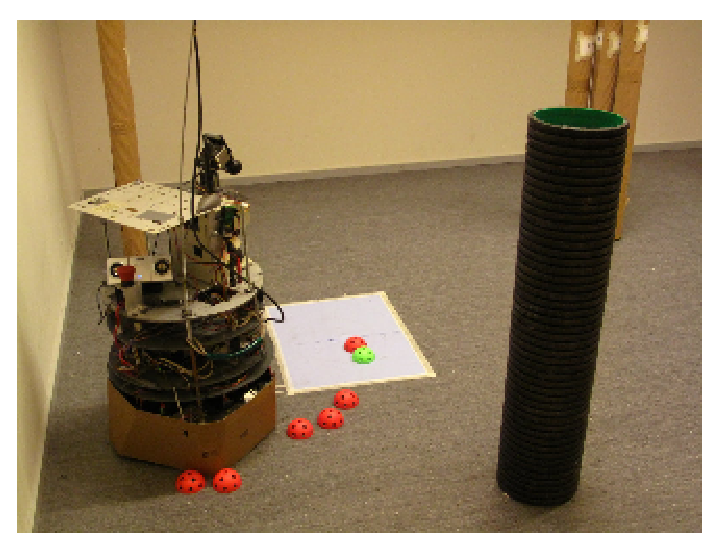
\includegraphics[width=8.0cm]{fail.eps}
\caption{A not so successful final placement of the targets (and an unwanted target).}
\label{fail} % The label for the figure. You can refer to the figure by \ref{fig:1} in the text. 
\end{center}
\end{figure}

\begin{figure}[!]	% Use here 'h' for 'here', 't' for 'top' or 'b' for bottom. '!' makes the figure float.
\begin{center}
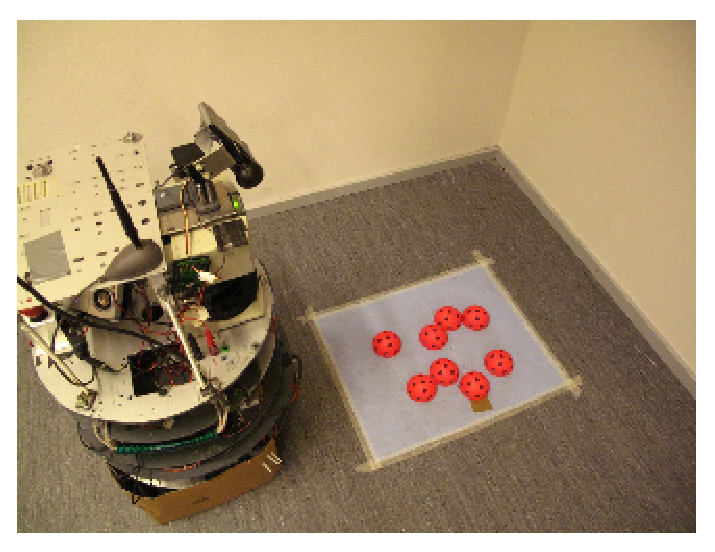
\includegraphics[width=8.0cm]{success.eps}
\caption{A very successful final placement of the targets.}
\label{success} % The label for the figure. You can refer to the figure by \ref{fig:1} in the text. 
\end{center}
\end{figure}

\section{Project Management}

The project team had weekly meetings for keeping everyone up-to-date. The work was divided so that one person was mainly responsible for one subtask, but also one or two other persons were assigned for the same subtask. The division of the work can be seen in table \ref{Division_of_work}.

\subsection{Time Usage}


\begin{table}[!ht]
\begin{scriptsize}
\caption{Division of work. Persons mainly responsible in each area marked in bold.}
\label{Division_of_work}
\begin{tabular}{|l|l|l|l|l|l|l|l|}
\hline
 &Manipulator&SLAM&Navigation&Motion&Object&Planner&Documenting\\

  &&&&Control&recognition&&\\
 \hline
Konsta & & & \textbf X & X & & X & X \\ \hline
Antti & & \textbf X &  &  & &  & \\ \hline
Iiris & & & & \textbf X & & X & X \\ \hline
Toni & & & & & \textbf X &  &  \\ \hline
Hanna & X & & & X & & & \textbf X \\ \hline
Pekka & \textbf X & & & X & & X & \\ \hline
Quentin & X & & & X & & & X \\ \hline
\end{tabular}
\end{scriptsize}
\end{table}


On average, 75 hours (2.8 credits) were used to the project per person. However, there are somewhat large variations. One of the main challenges regarding the division of work was, that the programming tasks required a good amount of C$++$ skills, and as some of the group members weren't that proficient in C$++$, the programming tasks were focused on those who could program. This can be seen from the fact that the people responsible for programming tasks spent on average roughly 100 hours (3.7 credits) per person, whereas the others spent on average only roughly 45 hours (1.7 credits). 


In the future, it would be good that the C$++$ course would be a prerequisite of this course, as this would make dividing work equally much easier. Also the general workload of this project work is roughly 40$\%$ more than the indicated 2 credits. As, based on the project experience, the given task couldn't have been done in a 2 credit project, in the future one or more of the following actions should be taken by the course personnel:
\begin{itemize}
\item Change project so that it takes less time to implement by

\begin{enumerate}
\item giving less or easier functional requirements
\item having a programming environment which takes less time to configure (this could be done when the new Pioneer platform is used)
\item allocating more people per group (e.g.with 10 people 550 man-hours equals roughly 2 credits per person)
\end{enumerate}

\item Allocate sufficient credits for the project (i.e. one credit more)
\end{itemize}


The man-hours (mh) were roughly divided as follows:

\begin{center}

\begin{tabular}{l|l|l}


General activities* & 135 mh & 	25$\%$ \\
Manipulator & 44 mh	& 8$\%$ \\
SLAM	 & 70 mh	 & 13$\%$ \\
Object recognition & 86 mh & 16$\%$ \\
Navigation & 52 mh & 10$\%$ \\
Movement control & 58 mh	 & 11$\%$ \\
Operation planning & 38 mh &7$\%$ \\
Documentation (estimate)	 & 60 mh & 11$\%$ \\
Total & 543 mh & 100$\%$ \\

\end{tabular}
\end{center}

*meetings, setting up programming environments, demos, other programming, "anything else"\\

It can be seen that all the different modules took roughly the same amount of work. 


Setting up programming environments (such as making our own build system, installing all the required libraries to everyone and getting them to work) was quite laboursome and did not actually contribute to the learning objectives of this course. If this work could be lessened, more time and effort could be directed to programming actual functionality. Retrospectively, general activities could have been divided into two or more separate categories to illustrate this better.


The total work done was tracked on a day-to-day basis, and the data is visualized in figure \ref{man_hours}. It can be seen that at the beginning the majority of the work went to documentation and general activities. After the first weeks, movement control, object recognition and manipulator started to gain hours as well alongside general activities, whereas documentation work stopped. After the first month navigation and SLAM started also to progress. The work was divided quite evenly throughout the project timeline, although there is a large spike just before the final demo date. It can be also noticed that the operation planning implementation started only a few weeks before the final demo. It is quite clear that the operation planning implementation should have been started earlier, but the reason for this was that there simply was not enough programming man-hours available before some of the other functionality was finished.

\begin{figure}[h]	% Use here 'h' for 'here', 't' for 'top' or 'b' for bottom. '!' makes the figure float.
\begin{center}
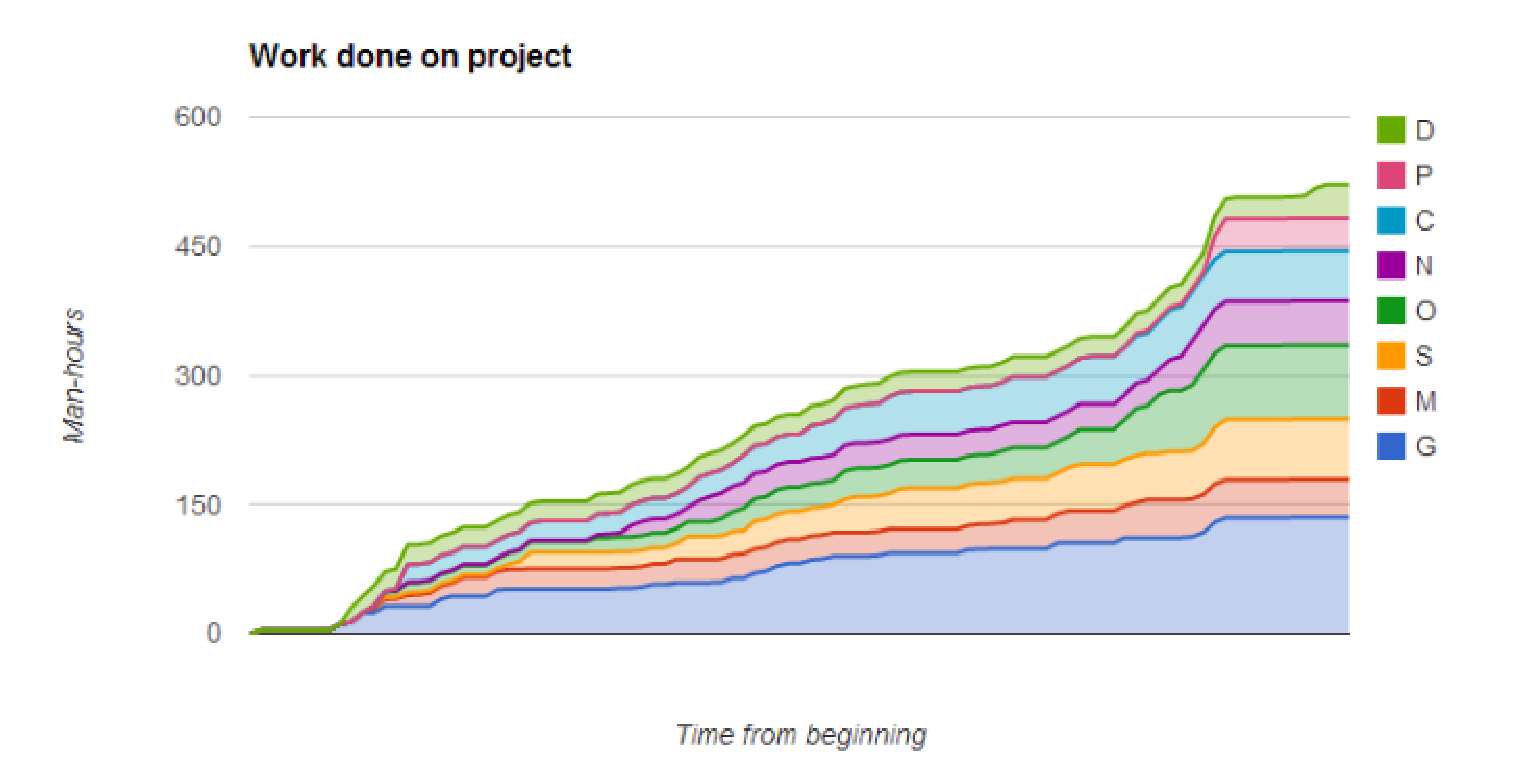
\includegraphics[width=10.0cm]{man_hours.eps}
\caption{Man-hours used in project as a function of time, divided according to subcategory (Documenting, operation Planning, movement Control, Navigation, Object recognition, Slam, Manipulator, General activities). Not all of documentation was finished when this image was generated.}
\label{man_hours} % The label for the figure. You can refer to the figure by \ref{fig:1} in the text. 
\end{center}
\end{figure}

\section{Conclusions}

The project was finished rather successfully in time. After fixing the bug from last night coding, the robot was able to collect 6/10 targets with 1 non-target. Robot localization worked well, and robot successfully navigated the paths between the walls and around the corners. The speed of the robot was rather slow, but faster speed could have caused problems with collected targets, since they might have prevented the wheels from moving correctly. Speed was also comparable to the other contestants' speeds.

The robot locates itself using the odometry data from the wheels and laser data in SLAM module, which creates a four-layered map where each layer contained different information; walls and empty areas, targets, not interesting targets and the goal area. Navigation algorithm finds the shortest path to the location, which causes the robot to move very close to the walls. Because turning of the robot was problematic due to caster wheels, the navigation could have been made better by tuning the path planning so that straight paths are favoured.

Motion control between the waypoints is very simple, with just P-controller for the turning speed and the coefficient that slow the movement down if large turns are needed. More sophisticated method could have been used to make the movement smoother.

The object recognition was done using the color information of the camera images. This caused some initial problems, because robot’s power cable had the same color as the targets. However, with proper post-processing of the image, the targets and non-targets were identified correctly. The calibration of the camera ensured that the calculated position of the target was very accurate when the target was near the center of the camera, and accurate enough to be useful even if the target lay near the edge of the image.

Two different manipulators were created. The first, called "Hatch" is basic in its design. It works perfectly in our situation and could be quickly implemented. The second design “Coffee gripper” has completely different look. This design, more ambitious, had to be abandoned because it only works when picking small objects. Due to lack of time, it has not been completely successfully in our project.

As the robot was represented as a circular object in its internal map, the deformity in this circle caused by the hatch and the servo was not easily accounted for in the short time between noticing the problem and the final demonstration. Pushing for full system testing earlier would have revealed the problem.

In project management point of view, we avoided a lot troubles with integration of the modules by designing the interfaces beforehand and implementing first very simple modules with little functionality. In so doing it was possible to incrementally add functionality to the modules (especially when using Git) and integrating the modules little by little.

The greatest challenges in the project were the division of the work, when group members had very different backgrounds and skills, and timing of the project. We had several parts ready for weeks before the final demo (SLAM, manipulator), but did not test them until the rest of the modules were ready. Testing should have been started earlier, even though some time would have been needed for setting up proper testing environment without the rest of the modules. We also learned that last night major changes in program are not a good thing without a proper testing.



%\begin{figure}[h]	% Use here 'h' for 'here', 't' for 'top' or 'b' for bottom. '!' makes the figure float.
%\begin{center}
% \includegraphics[width=5.0cm]{fsm.eps}
%\caption{Finite state machine to describe the robot's control logic.}
%\label{fig:fsm} % The label for the figure. You can refer to the figure by \ref{fig:1} in the text. 
%\end{center}
%\end{figure}


\bibliographystyle{mystyle_doi_isbn_en}
%\bibliographystyle{plain}
\bibliography{bibliography}

\begin{appendices}
\newpage
\section{Main Algorithms for SLAM}
\label{apA}

This section describes some of the main algorithms used by the SLAM module. They are in no particular order, but the relevance of each is explained and a simplified pseudo-code version of the algorithm is presented.

\subsection{SLAM::updateLaserData}

The purpose of this algorithm is to receive laser measurements from other modules and to send them to the gmapping wrapper. If gmapping does an update, this algorithm will update it to the current SLAM map.

\begin{verbatim}
updateLaserData(laserData):

if (laserData array is empty OR odometry not yet available) {
    // measurement array may be empty if the device is not
    // on or has some fault, odometry not yet available means
    // that the first laser measurement arrived before the first
    // odometry update
    print error
    return false
}

mapObject = empty map object
robotLocation = empty robot location

slamWrapper.update(latest laser data,
	latest location estimate,
	reference to mapObject,
	reference to robotLocation)

if (mapObject is updated) {
    if (this was the first SLAM update) {
        x0 = robotLocation.x - half map gridSize
        x1 = robotLocation.x + half map gridSize
        y0 = robotLocation.y - half map gridSize
        y0 = robotLocation.y + half map gridSize
        // we define the area of interest in the (quite large) map
        // given to us by the algorithm by putting the robot in
        // the center of the area of interest
    }
    
    robotLocation -= (x0, y0)
    currentMap.setGridLocation(robotLocation)
    // the location is defined relative to the area of interest
    
    // copy the data from the area of interest from the mapObject
    // to the currentMap
    for (x = x0 .. x1) for (y = y0 .. y1) {
    		currentMap.setCellValue(Location(x-x0, y-y0),
    		WALL, mapObject(x,y))
    	}
    	
    	<overwrite the surroundings of the initial location as free terrain and as goal area>

}    
\end{verbatim}

\subsection{SLAM::updateOdometryData}

The purpose of this method is to receive odometry measurements and update the current position estimate based on them. The measurements are integrated form, so they are not directly compatible with the current position, as they contain also integrated errors that are periodically corrected by the SLAM algorithm. Thus the module uses a static variable to create differential odometry measurements, which can then be integrated after they are rotated correctly (to be compatible with the current orientation).

\begin{verbatim}

updateOdometryData(RobotLocation loc):

static RobotLocation lastLoc

if (first odometry update) {
	lastLoc = loc
}

// dxy is the difference in two last raw odometry positions
// rotated so that theta is zero (in robot coordinates, sort of)
RobotLocation dxy = loc - lastLoc
dtheta = dxy.theta
dxy = dxy rotated -dtheta radians

// lastOdometryData is the odometry data given to the SLAM module, 
// and it needs to be continuous. So here we just integrate the 
// previous differences. Thus lastOdometryData should be pretty much 
// just the original odometry data minus a possible initial constant
double lastMeasurementTheta = lastOdometryData.theta
RobotLocation dxyo = dxy rotated lastMeasurementTheta radians 
dxyo.theta = dtheta
lastOdometryData += dxyo

// And here we integrate the differential on top of the current 
// location estimate, which is corrected every now and then by the 
// SLAM algorithm, so it may have discontinuities here and there
RobotLocation mapLoc = currentMap.getRobotLocation()
double currentTheta
RobotLocation dxym = dxy rotated currentTheta radians
dxym.theta = dtheta
mapLoc += dxym
currentMap.setLocation(mapLoc)

// store the last location for next time
lastLoc = loc

\end{verbatim}

\subsection{SLAM::updateImageData}

The purpose of this method is to receive image data objects and to keep track of the various objects that are observed using the camera (targets, obstacles and goal area). The different objects are stored in lists inside the MapData object as well as in occupancy grid format.

\begin{verbatimtab}
updateImageData(ImageData data, ObservationType type):

// first we reduce the observed area a small bit to lessen some 
// noticed edge effects
data.viewWidth -= 5 degrees
data.minDist += one grid cell size
data.maxDist -= one grid cell size

// the iteration limits
double thetaMin = data.location.theta - 0.5*data.viewWidth
double thetaMax = data.location.theta + 0.5*data.viewWidth
double r0 = 0.2 // minimum possible distance
double rMin = data.minDist
double rMax = data.maxDist

// iteration step sizes are scaled down a bit to make the iteration 
// more dense so that no cells in between are skipped. The angle step 
// for iteration is set so that even in the far end of the view 
// sector all occupancy grid squares are hit.
double dtheta = 0.8 * MapData::unitSize/data.maxDist
double dr = 0.8 * MapData::unitSize

// the treshold in distance to an existing target for creating a new 
// target instead of updating the location of an old one
double maxObjectDelta = MapData::unitSize * 2

// object lists (old-and-existing and old-to-be-deleted)
vector<Location> objects = copy currentMapData.getObjects(type)
vector<Location> trash = empty vector

for(theta = thetaMin:dtheta:thetaMax) for (r = r0:dr:rMax) {
	// iteration position
	double x = data.location.x + r*cos(theta)
	double y = data.location.x + y.sin(theta)
	
	// when we hit a wall in the iteration along a certain angle, 
	// the rest of the positions in this direction are occluded and
	// are thus not updated.
	double wall = currentMap.getValue(Location(x,y), WALL)
	if (wall > 0.5) {
		break // next theta
	}
	
	// the same happens if we see to a position that has not been 
	// yet seen by the laser (it could be a wall, so we are careful
	// not to jump into conclusions)
	if (wall < -0.5) {
		break // next theta
	}
	
	// we only update cells that are in the seen area, of course. 
	// however, we can't start the iteration from rMin as there may
	// we walls between the robot and rMin
	if (r < rMin) {
		continue // next r
	} 
	
	// we check what there is currently
	double oldValue = currentMap.getValue(Location(x,y), type)
	
	if (oldValue < 0.5) {
		// there is nothing here
		currentMap.setValue(Location(x,y), type, 0.0)
	}
	else {
		// there is something here
		if (type == GOAL) {
			// goal points are redrawn later
			currentMap.setValue(Location(x,y), type, 0.0)
		}
		
		if (type == TARGET || OBSTACLE) {
			// first let's find the object that corresponds to 
			// this location from the list of existing objects
			for (obj in objects) {
				if (obj is farther than maxObjectDelta) {
					continue // next obj
				}
				
				// then let's check if we still see this 
				// object or has it dissapeared
				bool newObjectExists = false
				for (obj2 in data.targets and trash) {
					if (obj2 is farther than maxObjectDelta) {
						continue // next obj2
					}
					newObjectExists = true
					if (obj2 is in data.targets) {
						// ignore this measurement as an old 
						// targets exists already
						add obj2 to trash
						delete obj2 from data.targets
					}
				}
				if (newObjectExists == false) {
					// no new observation, so this object has 
					// dissappeared and is removed
					delete obj from objects
				}
				
				// se this to 0 to avoid double tagging this 
				// grid cell, it will be redrawn later if there 
				// still is an object here
				currentMap.setValue(Loc(x,y), type, 0.0)
				
				// there should not be any other objects nearby
				break
			}
		}
	}
}

// after iteration, all the objects in data.targets should be new
// objects that we haven't seen before, but first check if they are
// in unprobable locations that we can discard
for (obj in data.targets) {
	if (location of object contains wall) {
		delete obj from data.targets
	}
}

// as some of the old targets may have gotten under the robot, we 
// will not track them any more
for (obj in objects) {
	if (location of object under robot radius of current location) {
		delete obj from objects
	} 
}

// now we can finally integrate the old objects with the new ones, 
// this is done a bit differently for different types
if (type == TARGET || OBSTACLE) {
	for (obj in data.targets) {
		
		// double check for duplicates
		bool duplicate = false
		for (obj2 in objects) {
			if (obj closer than maxObjectDelta to obj2) {
				duplicate = true
				break
			}
		}
		
		// if really a new object, add to old objects
		if (duplicate = false) {
			add obj to objects
		}
	}
}

// the data.targets for goals should contain all the identified 
// corner points. however, if there are more or less than 4, we will
// not accept this measurement
if (type == GOAL && data.target.size == 4) {
	check that the corner points form roughly a correct size and 
	shape of goal area
	
	if (goal area is ok) {
		clear targets
		add goal center point to objects
		add four corner points to objects
	}
}

// now all the data in the lists should be up to date, then we only 
// have to redraw the objects to the occupancy grid
if (type == TARGETS || OBSTACLES) {
	for (obj in objects) {
		currentMap.setValue(location, type, 1.0)
	}
}

if (type = GOAL) {
	if (objects.size = 5) {
		draw square based on corner points
	}
	else {
		draw circle to the initial location
	}
}

// update to the current MapData
currentMap.setObjects(objects, type)
\end{verbatimtab}


\end{appendices}

\end{document}
